\documentclass[../main.tex]{subfiles}
\begin{document}
\subsection{Numerical results}\label{subsec:results}

In the following we will solve the non-autonomous system \eqref{eq:nonautonomous_shifted} for different values of the shift ramp $\varepsilon>0$ and infere qualitatevely how it affects the properties of the a set of solutions. 

We truncate the time domain to be finite, i.e. we choose $T>0$ so that $\{-T,T\}$ represents the time horizons for the past and future limit systems.

\begin{figure}[H]
    \begin{subfigure}[b]{0.495\textwidth}
        \centering 
        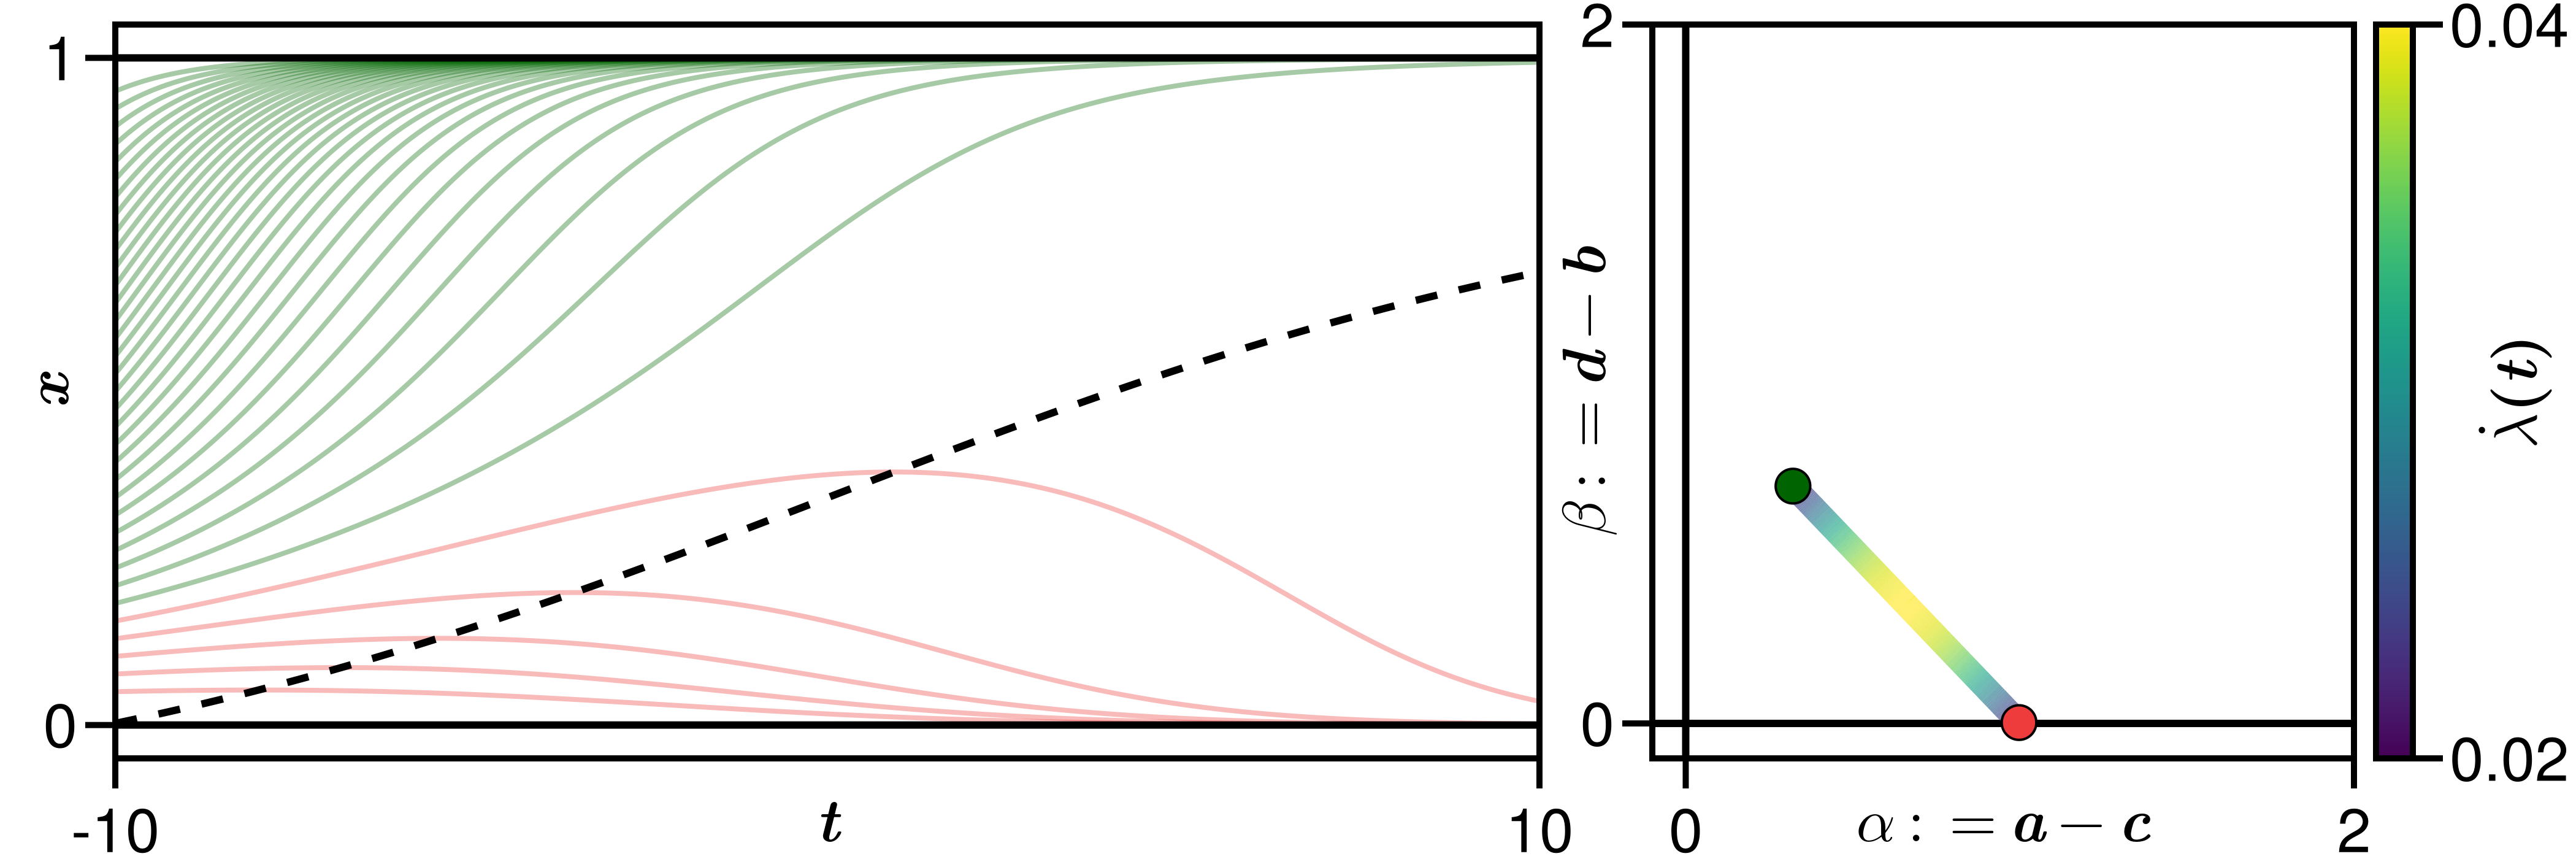
\includegraphics[keepaspectratio, width = \linewidth]{../figures/fig:nonautonomous_1.png}
        \caption{$\varepsilon = 0.15$}
        \label{fig:nonautonomous_1}
    \end{subfigure}
    \hfill
    \begin{subfigure}[b]{0.495\textwidth}
        \centering 
        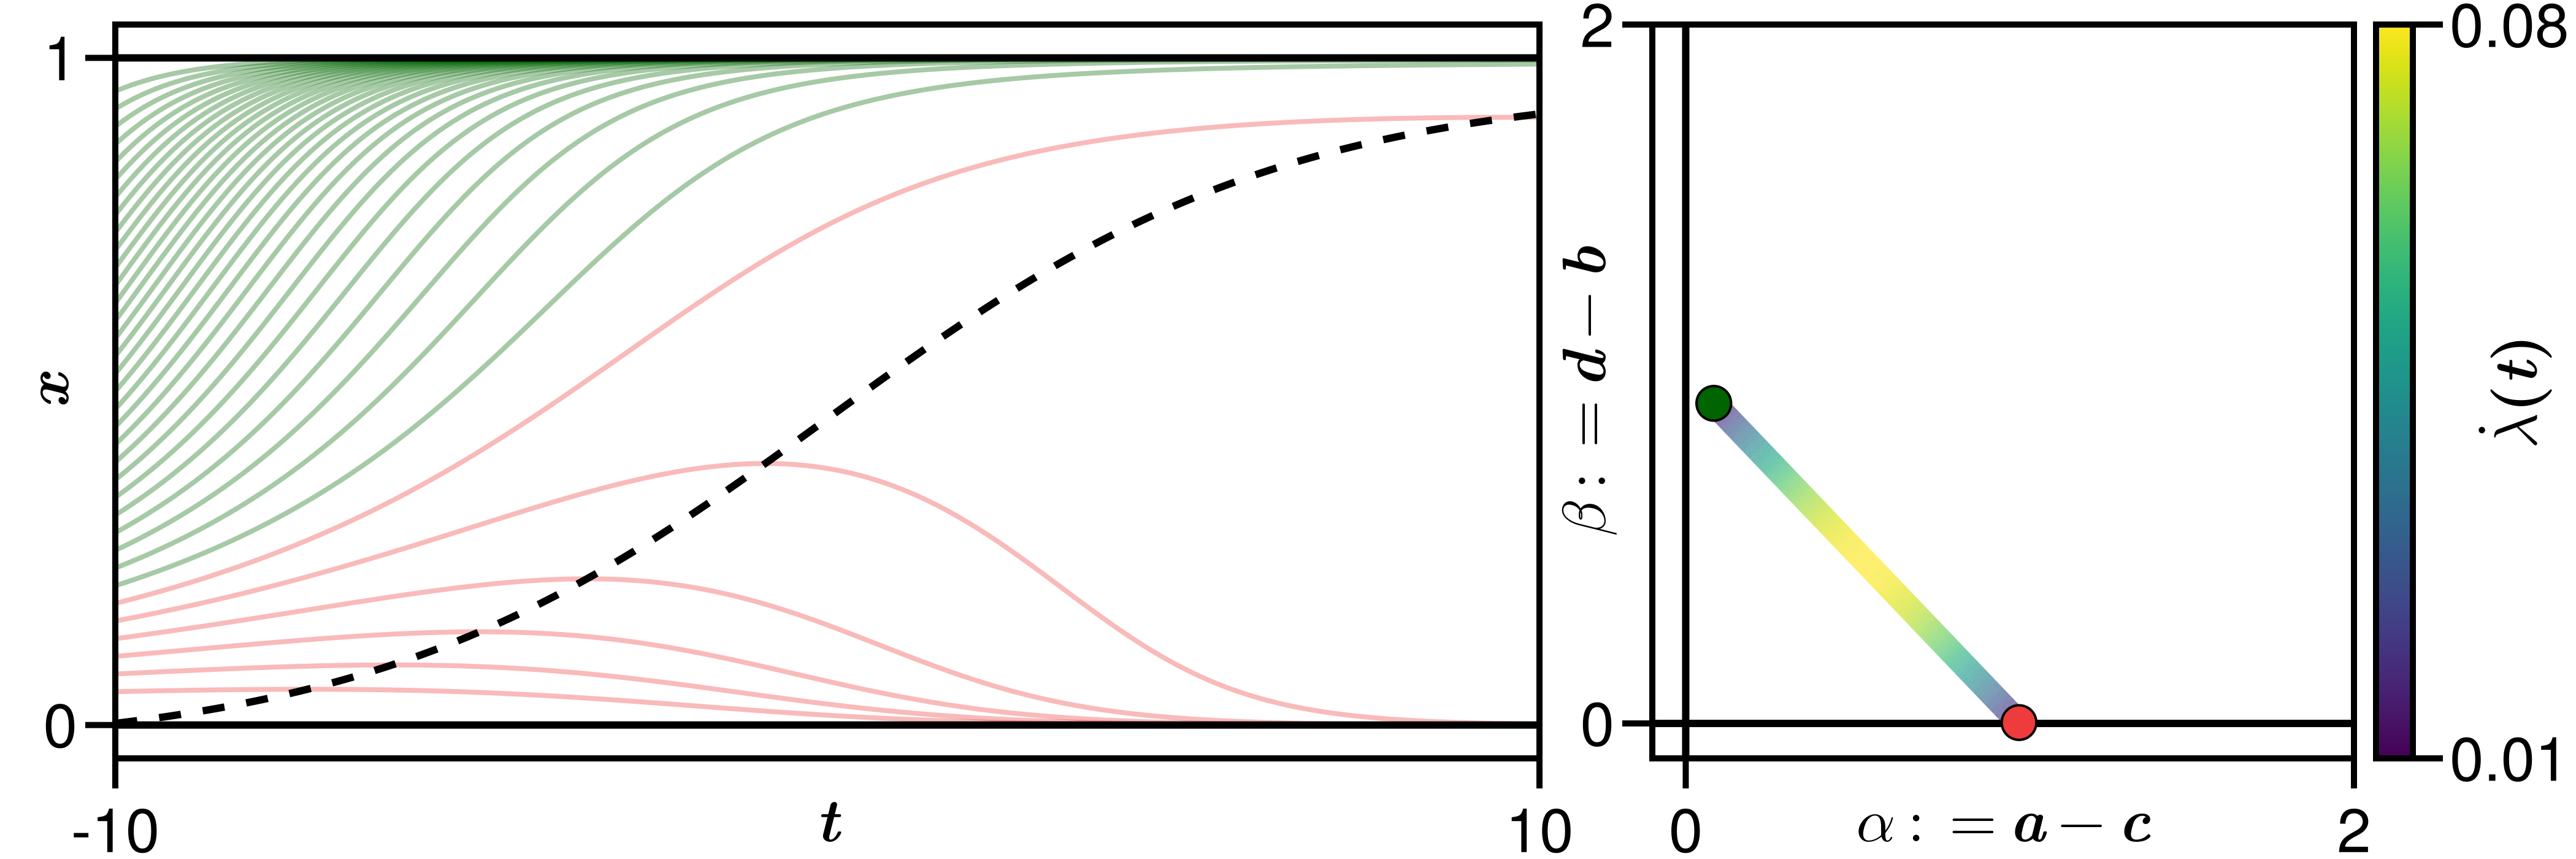
\includegraphics[keepaspectratio, width = \linewidth]{../figures/fig:nonautonomous_2.png}
        \caption{$\varepsilon = 0.2$}
        \label{fig:nonautonomous_2}
    \end{subfigure}

    \begin{subfigure}[b]{0.495\textwidth}
        \centering 
        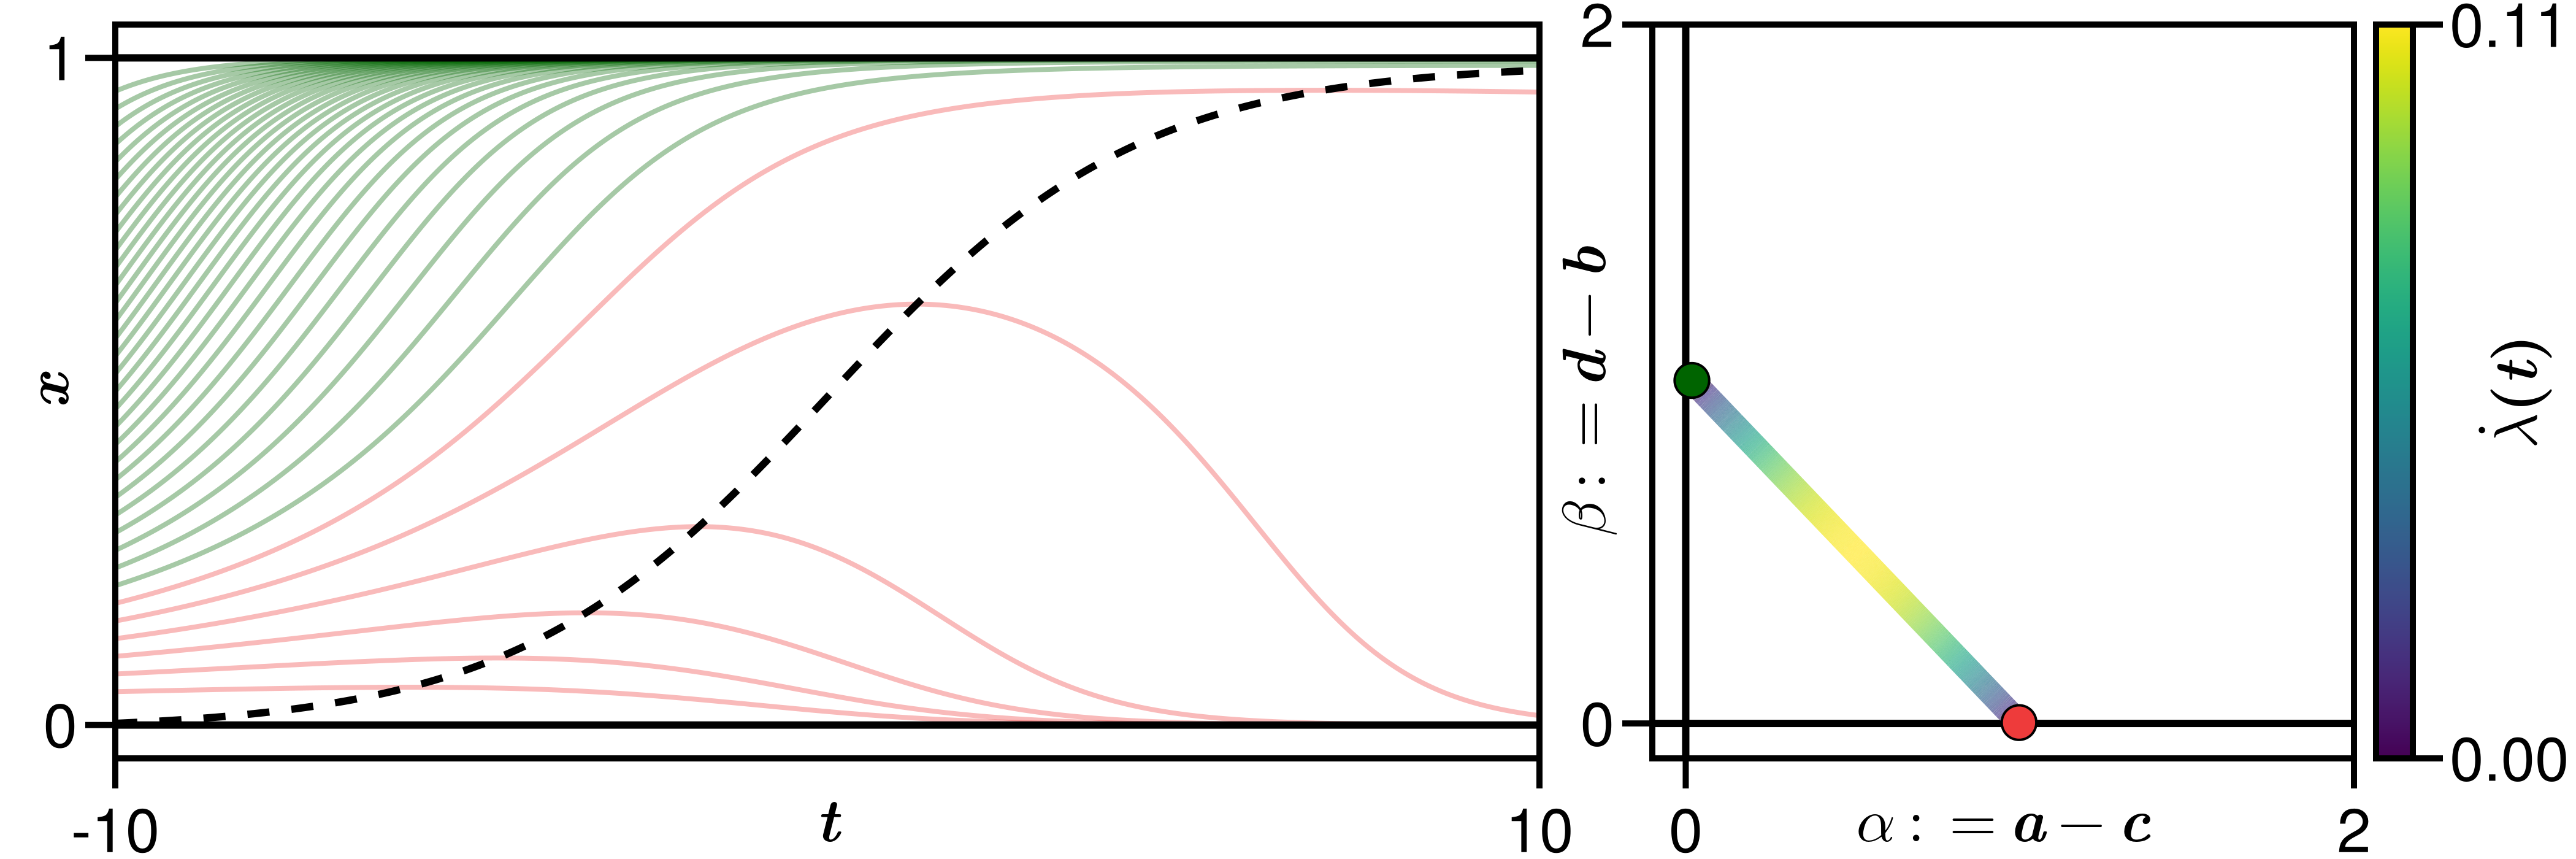
\includegraphics[keepaspectratio, width = \linewidth]{../figures/fig:nonautonomous_3.png}
        \caption{$\varepsilon = 0.25$}
        \label{fig:nonautonomous_3}
    \end{subfigure}
    \hfill
    \begin{subfigure}[b]{0.495\textwidth}
        \centering 
        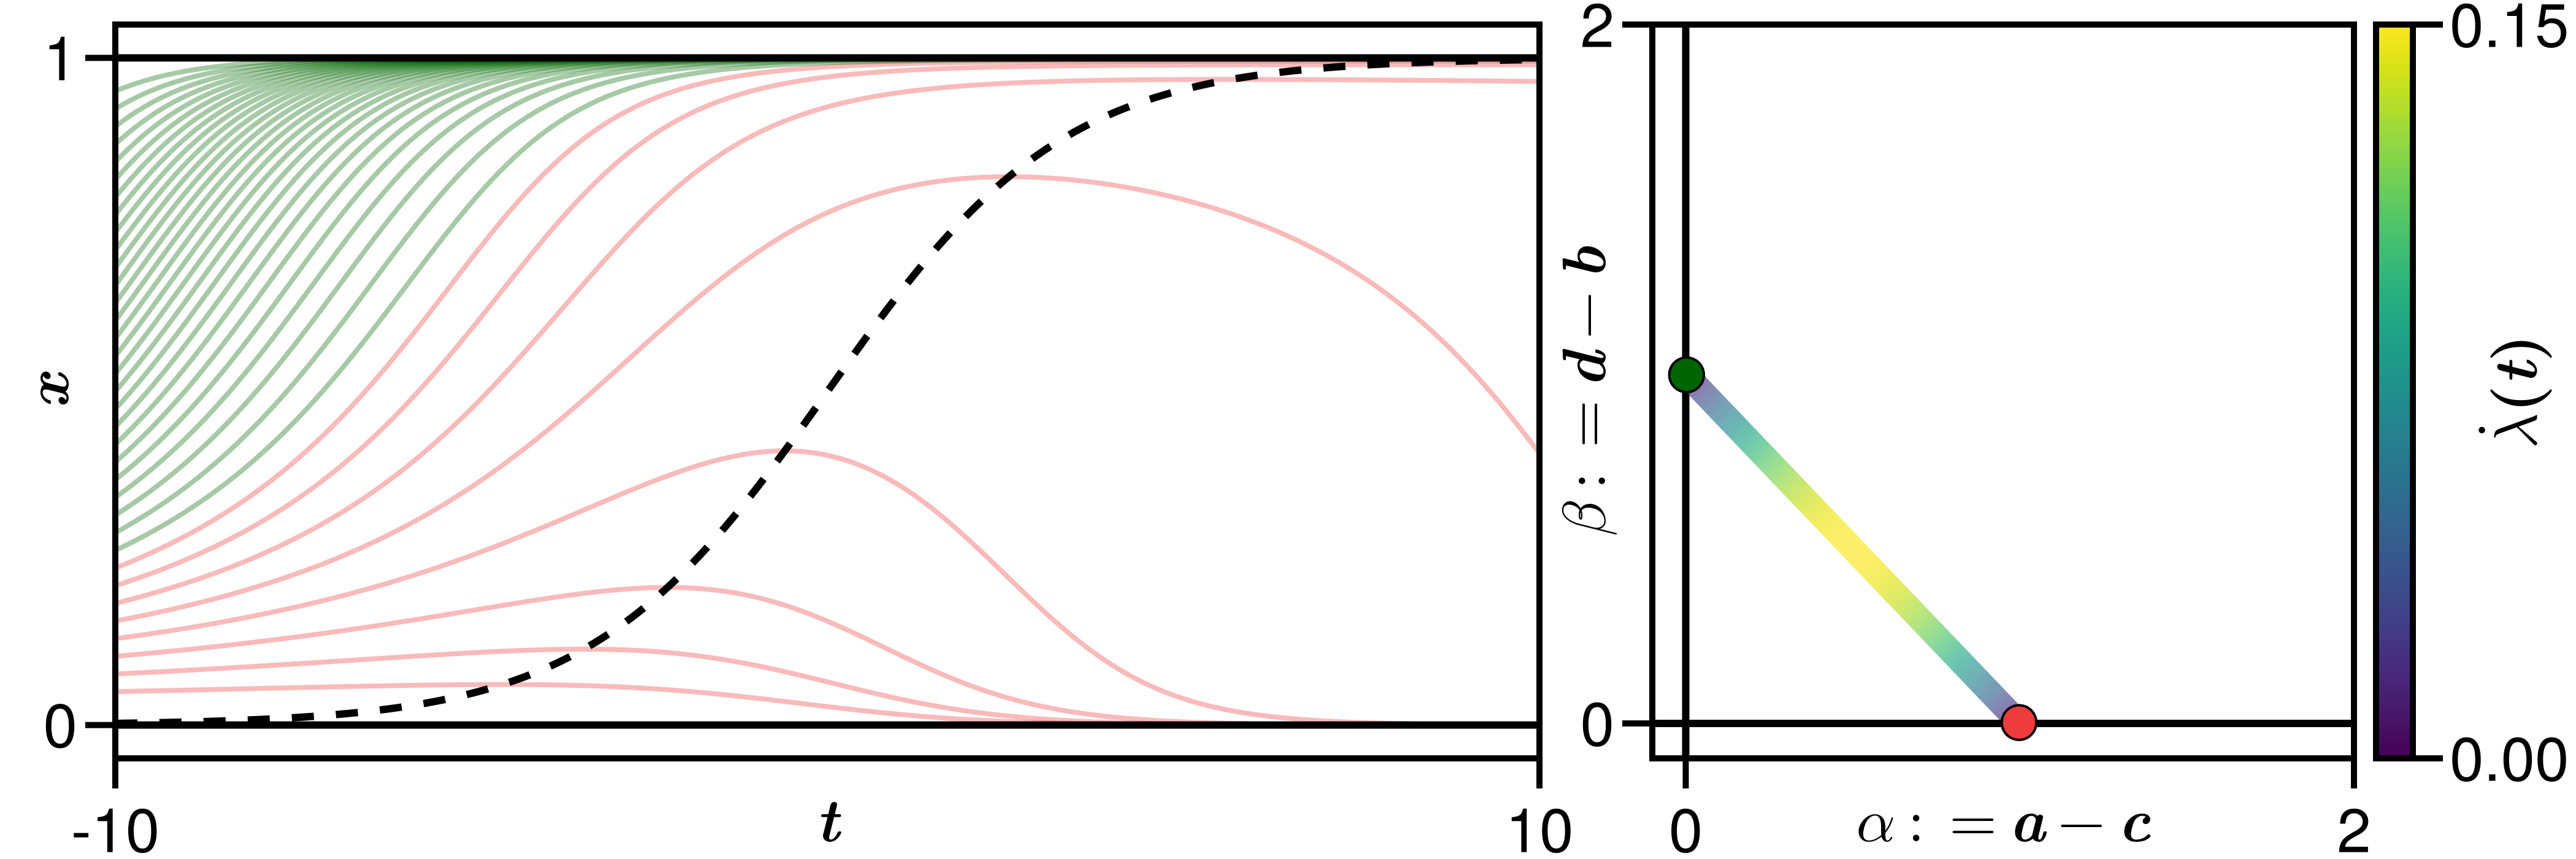
\includegraphics[keepaspectratio, width = \linewidth]{../figures/fig:nonautonomous_4.png}
        \caption{$\varepsilon = 0.3$}
        \label{fig:nonautonomous_4}
    \end{subfigure}

    \caption{Solutions of the non-autonomous replicator system with a hyperbolic tangent shift of the parameter formulated in \eqref{eq:nonautonomous_shifted}.
            Different shift rates $\varepsilon$ are depicted with increasing values sorted left to right and top to bottom (the values for $\varepsilon$ are reported in the caption of each subplot).
            The time truncation is set to $T=10$ and we set the $\delta=0$ so that the shift's time derivative is maximised at time $t=0$.
            For each subplot the left (rectangular) box displays the timeseries of solutions of a set of initial conditions in $\mathbb{B}(x_{2},-T)$: green lines indicate those solutions that have not undergone R-tipping at time $T=10$, red lines those that did, black solid lines indicate the stable equilibria $x_{1}$, $x_{2}$ and the dashed black line indicate the unstable equilibria $x_{*}$.
            Conversely the right (square) box indicates the trajectory of the shifted parameter $\lambda(t) = \beta = 1 - \alpha$ in $\tilde{\Gamma_{*}}$ from its past limit value (red dot) to its future limit value (green dot). 
            The color along the curve indicates the magnitude of its rate of change at different timesteps (i.e. the value of $\dot{\Lambda}(t)$) as encoded on the colorbar on the left.
    }
    \label{fig:nonautonomous}
\end{figure}

\end{document}
